\section{Relationship between the rank CDF of positives and contingency tables} \label{rank-roc}
The challenge of incorporating unlabeled data into an evaluation metric is knowing which unlabeled examples are latent positives and which are latent negatives. Our insight is that, if the known positives are sampled completely at random from all positives, the rank distribution of latent positives should follow the rank distribution of known positives. Thus if we know $\pfrac$, which is needed to compute the expected number of latent positives within the unlabeled data, this provides an avenue for building contingency tables that incorporate the unlabeled data. To do so, we first prove relationships between rank CDFs of sets of positives within an overall ranking at a given rank $r$ and the corresponding contingency tables. Then, we use these relationships to prove bounds on the FPR at a given rank $r$ when the ranking includes unlabeled examples, some of which are latent positives. 

%The challenge of incorporating unlabeled data into an evaluation metric is knowing which unlabeled examples are latent positives and which are latent negatives. Our insight is that, if the known positives are a random sample from all positives, the rank CDF of the latent positives should follow the rank distribution of the known positives. This assumes that we know $\beta$ as we need to compute the expected number of latent positives within the unlabeled data. To do so, we first prove relationships between the rank CDFs of sets of positives within an overall ranking at a given rank $r$ and the corresponding contingency table. Then, we use these relationships to prove bounds on the FPR at a given rank $r$ when the ranking includes unlabeled examples, some of which are latent positives. 

%These relationships allow us to efficiently estimate contingency tables based on an overall ranking $\overall$, a subset of known positives $\knownpos$ and an estimate $\hat{\pfrac}$ in Section~\ref{practical}. 

%%%%%%%%%%%%%%%%%%%%%%%%%%%%%%%%%%%%%%%%%%%%%%%%%%
% 	LEMMA RANK -> FPR
%%%%%%%%%%%%%%%%%%%%%%%%%%%%%%%%%%%%%%%%%%%%%%%%%%

\subsection{Rank distributions and contingency tables based on subsets of positives within a ranking}
We begin by considering given sets of positives within an overall ranking. Proofs of all lemmas can be found in Appendix~\ref*{proofs}, along with figures to illustrate the associated property.

\begin{replemma}{lemma-rank-fpr}
Given a rank $\ranksymb$ and two disjoint subsets of positives $\pos_1$ and $\pos_2$ within an overall ranking $\overall$. If $|\pos_1|=|\pos_2|$ and $\TPR(\pos_1, \ranksymb) > \TPR(\pos_2,\ranksymb)$, then $\FPR(\pos_1,\ranksymb) < \FPR(\pos_2,\ranksymb)$. If $\TPR(\pos_1, \ranksymb) = \TPR(\pos_2,\ranksymb)$, then $\FPR(\pos_1, \ranksymb) = \FPR(\pos_2,\ranksymb)$.
\end{replemma}


%%%%%%%%%%%%%%%%%%%%%%%%%%%%%%%%%%%%%%%%%%%%%%%%%%
% 	LEMMA RANK UNION
%%%%%%%%%%%%%%%%%%%%%%%%%%%%%%%%%%%%%%%%%%%%%%%%%%

\begin{replemma}{lemma-rank-union}
Given a rank $\ranksymb$ and two disjoint sets of positives $\pos_1$, $\pos_2$ in a ranking $\overall$ and $\bothpos=\pos_1\cup\pos_2$. If $\TPR(\pos_1,\ranksymb) < \TPR(\pos_2, \ranksymb)$ then $\TPR(\pos_1,\ranksymb) < \TPR(\bothpos,\ranksymb) < \TPR(\pos_2, \ranksymb)$.
\end{replemma}

\begin{repcorollary}{corollary-rank-union}
Given a rank $\ranksymb$ and three sets of positives $\pos_A$, $\pos_B$ and $\pos_C$ within a ranking $\overall$ such that $\pos_A\cap\pos_B=\emptyset$ and $\pos_A\cap\pos_C=\emptyset$ and $|\pos_B|=|\pos_C|$, then
\begin{equation*}
\TPR(\pos_B,\ranksymb) < \TPR(\pos_C,\ranksymb) \quad\leftrightarrow\quad \TPR(\pos_A\cup \pos_B,\ranksymb) < \TPR(\pos_A\cup\pos_C,\ranksymb).
\end{equation*}
%\textbf{Proof}: all terms are equal for $\TPR(\pos_A\cup \pos_B,\ranksymb)$ and $\TPR(\pos_A\cup \pos_C,\ranksymb)$ except $\tprsymb_B < \tprsymb_C$ in Eq.~\eqref{tpr-union}.
\end{repcorollary}

% TODO
\ifx
\begin{figure}[!h]
  \centering
  \RawFloats
  \begin{minipage}[b]{0.49\textwidth}
  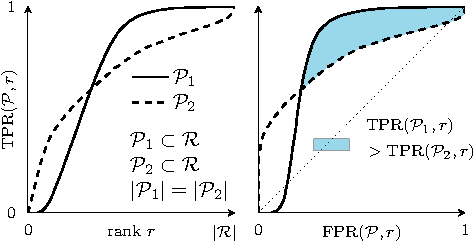
\includegraphics[width=\textwidth]{lemma_rank_fpr.pdf}
  \caption{Illustration of Lemma~\ref{lemma-rank-fpr}: higher TPR at a given rank $r$ implies lower FPR at $r$ for two positive sets of the same size.}
  \label{fig:lemma-rank-fpr}
  \vfill
  \end{minipage}
  \hfill
%\end{figure}
%\end{minipage}
%\begin{minipage}[0.47\textwidth}
%\begin{figure}[!h]
%  \centering
  \begin{minipage}[b]{0.49\textwidth}
  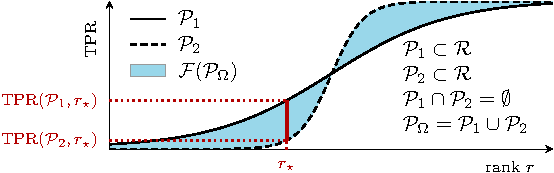
\includegraphics[width=\textwidth]{lemma-rank-union.pdf}
  \caption{Illustration of Lemma~\ref{lemma-rank-union}: $\mathcal{F}(\cdot)$ denotes feasible region. The rank distribution of the union $\bothpos$ of two sets of positives $\pos_1$ and $\pos_2$ lies between their respective rank distributions.} 
  \label{fig:lemma-rank-union}
\vfill
  \end{minipage}
\end{figure}
%\end{minipage}
\fi

\subsection{Contingency tables based on partially labeled data}
Lemmas~\ref*{lemma-rank-fpr} and \ref*{lemma-rank-union} describe relationships between rank distributions and contingency tables of different (but known) sets of positives within an overall ranking. 
%However, computing contingency tables from partially labeled data requires accounting for the unknown set of latent positive examples $\latentpos$ in the unlabeled data, that is, $\bothpos = \knownpos \cup \latentpos$, such that $|\latentpos| > 0$ and $|\latentpos|=\pfrac\cdot|\unlabeled|$. 
We now show how to construct contingency tables corresponding to the greatest-lower and least-upper bound of the FPR at a given rank, accounting for the unknown set of latent positive example from partially labeled data, given $\pfrac$. 

%Assuming a known proportion of latent positive examples in the unlabeled data, 

%and prove that one corresponds to the greatest lower bound of the FPR and the other corresponds to the least upper bound of the FPR at a specified rank.  

%Assumming a known proportion of latent positive examples in the unlabeled data, we now show to construct two contingency tables from partially labeled data and prove that one corresponds to the greatest lower bound of the FPR and the other corresponds to the least upper bound of the FPR at a specified rank.  

%%%%%%%%%%%%%%%%%%%%%%%%%%%%%%%%%%%%%%%%%%%%%%%%%%
% 	THEOREM
%%%%%%%%%%%%%%%%%%%%%%%%%%%%%%%%%%%%%%%%%%%%%%%%%%

\begin{theorem} \label{main-theorem}
%Given an overall ranking $\overall = \knownpos \cup \knownneg \cup \unlabeled$, consisting of disjoint sets of known positives $\knownpos$, known negatives $\knownneg$ and unlabeled instances $\unlabeled$, where $\unlabeled$ contains an unknown set of latent positives $\latentpos \subset \unlabeled$ of known size $|\latentpos| = \pfrac \cdot|\unlabeled|$. Given a rank $\ranksymb$ and an upper bound $\mathcal{T}_{ub}(\ranksymb) \geq \TPR(\latentpos, \ranksymb)$, a tight lower bound on $\FPR(\bothpos, \ranksymb)$ with $\bothpos = \knownpos \cup \latentpos$ can be found without explicitly identifying $\latentpos$.
Given an overall ranking $\overall$ consisting of disjoint sets of known positives $\knownpos$, known negatives $\knownneg$ and unlabeled instances $\unlabeled$, where $\unlabeled$ contains an unknown set of latent positives $\latentpos \subset \unlabeled$ of known size $|\latentpos| = \pfrac \cdot|\unlabeled|$. Given a rank $\ranksymb$ and an upper bound $\mathcal{T}_{ub}(\ranksymb) \geq \TPR(\latentpos, \ranksymb)$, a tight lower bound on $\FPR(\bothpos, \ranksymb)$ with $\bothpos = \knownpos \cup \latentpos$ can be found without explicitly identifying $\latentpos$.


\textbf{Proof}: Step 1: assign a set of surrogate positives $\surrpos$:\footnote{A surrogate positive is an example that we treat as if its ground truth label is positive (even though in reality its ground truth label is unknown) when constructing a contingency table.}
\begin{align}
\surrpos = &\argmin_{\surrposopt\subset\ \unlabeled}\ \TPR(\surrposopt, \ranksymb), \label{eq:surrpos-def}  \\ 
&\subjectto\ \TPR(\surrposopt,\ranksymb) \geq \mathcal{T}_{ub}(\ranksymb) \text{ and } |\surrposopt|=\pfrac\cdot|\unlabeled|, \nonumber
\end{align}
then $\TPR(\surrpos,\ranksymb) \geq \TPR(\latentpos,\ranksymb)$ by construction. If $|\topfun(\unlabeled, r)| < \pfrac\mathcal{T}_{ub}(\ranksymb)\cdot |\unlabeled|$, then no $\surrpos$ exists that satisfies the constraint $\TPR(\surrpos, \ranksymb) \geq \mathcal{T}_{ub}(\ranksymb)$ in Equation~\eqref{eq:surrpos-def}.\footnote{An infeasibility implies that $\mathcal{T}_{ub}(\ranksymb)$ and/or $\pfrac$ are too high.} In this case, treat all instances in $\topfun(\unlabeled, \ranksymb)$ as surrogate positive, which trivially implies $\TPR(\surrpos, \ranksymb) \geq \TPR(\latentpos, \ranksymb)$.

Step 2: define $\bothposapprox = \knownpos \cup \surrpos$. Using Corollary~\ref{corollary-rank-union} yields $\TPR(\bothposapprox, \ranksymb) \geq \TPR(\bothpos, \ranksymb)$. Since $|\bothposapprox|=|\bothpos|$, using Lemma~\ref*{lemma-rank-fpr} yields the lower bound on FPR, i.e., $\FPR(\bothposapprox, \ranksymb) \leq \FPR(\bothpos, \ranksymb)$.\hfill$\blacksquare$
%\begin{align*}
%\FPR(\bothposapprox, \ranksymb) \leq \FPR(\bothpos, \ranksymb).\tag*{$\blacksquare$}
%\end{align*}
\end{theorem}

Applying Theorem~\ref{main-theorem} yields a nontrivial lower bound on $\FPR(\bothpos,\ranksymb)$. In Lemma~\ref*{lemma-glb} we prove that $\FPR(\bothposapprox,\ranksymb)$ is the greatest achievable lower bound based on a given $\unlabeled\subset\overall$.

\begin{replemma}{lemma-glb}
Minimizing $\TPR(\surrpos, \ranksymb)$ in Equation~\eqref{eq:surrpos-def} of Theorem~\ref{main-theorem} ensures $\FPR(\bothposapprox, \ranksymb)$ is the greatest achievable lower bound on $\FPR(\bothpos, \ranksymb)$ given $\pfrac$, $\mathcal{T}_{ub}(\ranksymb)$, $\overall$ and $\unlabeled$. 
\end{replemma}

Due to its symmetry, Theorem~\ref{main-theorem} can also be used to obtain the least achievable upper bound of $\FPR(\bothpos, \ranksymb)$ given a ranking $\overall$ and a bound $\mathcal{T}_{lb}(\ranksymb) \leq \TPR(\surrpos, \ranksymb)$ by assigning $\surrpos$ such that:
\begin{align}
\surrpos = &\argmax_{\surrposopt\subset\ \unlabeled}\ \TPR(\surrposopt, \ranksymb), \label{eq:surrpos-def-ub} \\
&\subjectto\ \TPR(\surrposopt,\ranksymb) \leq \mathcal{T}_{lb}(\ranksymb) \text{ and } |\surrposopt|=\pfrac\cdot|\unlabeled| \nonumber. 
\end{align}
%If this is infeasible (implying $\mathcal{T}_{ub}(\ranksymb)$ and/or $\pfrac$ are too low), use 
%\begin{equation*}
%\surrpos = \argmin_{\surrpos\subset\ \unlabeled} \TPR(\surrpos, \ranksymb). \label{eq:surrpos-alternative}
%\end{equation*}
